\documentclass[xcolor=dvipsnames,8pt]{beamer}
% ********** Styl prezentacji **********
\mode<presentation>
{
%\usetheme{Frankfurt}
%\usetheme{Copenhagen}
%\usetheme{Madrid}
\usetheme{Warsaw}
%\usetheme{lankton-keynote}
 %Copenhagen
}
%\usepackage{amsmath}
%\usepackage{amsthm}
%\usepackage{amsfonts}
\usepackage{color}
%\usepackage{listings}
%\lstset{language=C++}
%\usepackage{lscape} 
%\usepackage{float}
%\usepackage{graphicx}
\usepackage{caption}
\usepackage{subcaption}
%\usepackage{multimedia}
% common reference commands
\newcommand{\eqt}[1]{Eq.~(\ref{#1})}                     % equation
\newcommand{\fig}[1]{Fig.~\ref{#1}}                      % figure
\newcommand{\tbl}[1]{Table~\ref{#1}}                     % table
%\usepackage{movie15}
%\usepackage{hyperref}
%\usepackage{multimedia}
\usepackage[]{media9}
%\usepackage{filecontents,hyperref,listings}
\renewcommand{\div}{\vec{\nabla} \cdot}
\newcommand{\grad}{\vec{\nabla}}
\newcommand{\mbold}[1]{\boldsymbol#1}
\newcommand{\tcm}[1]{\textcolor{magenta}{#1}}
\newcommand{\tcr}[1]{\textcolor{red}{#1}}
\newcommand{\tcb}[1]{\textcolor{blue}{#1}}
\newcommand{\resi}{R}
\newcommand{\resinew}{\widetilde{\resi}}
\newcommand{\norm}{\textrm{norm}}
%
%\setbeamertemplate{footline}[frame number]
%\title{Extension of the entropy viscosity method to low Mach regime and the seven equations model.}
%\title{Extension of the entropy viscosity method to low Mach regime and the seven equations model.}
%\author{Marc-Olivier Delchini}
%
\date{11/11/2014}

%\addtobeamertemplate{footline}{\hfill\insertframenumber/\inserttotalframenumber\hspace{2em}\null}

\setbeamertemplate{footline}{
\leavevmode%
%\hbox{\hspace*{-0.06cm}
\begin{beamercolorbox}[wd=.5\paperwidth,ht=3.25ex,dp=1ex,center]{author in head/foot}%
	\usebeamerfont{author in head/foot}\insertshortauthor%~~(\insertshortinstitute)
\end{beamercolorbox}%
\begin{beamercolorbox}[wd=.25\paperwidth,ht=3.25ex,dp=1ex,center]{section in head/foot}%
	\usebeamerfont{section in head/foot} PHYSOR-2014 % \insertshorttitle
\end{beamercolorbox}%
\begin{beamercolorbox}[wd=.25\paperwidth,ht=3.25ex,dp=1ex,left]{section in head/foot}%
	\usebeamerfont{section in head/foot}\insertshortdate{}\hspace*{2em}
	\insertframenumber{} / \inserttotalframenumber %\hspace*{2ex}
\end{beamercolorbox}}%
%\vskip0pt%
%}

\beamertemplatetransparentcovered

\urldef{\ragusa}\url{jean.ragusa@tamu.edu}
\urldef{\delchini}\url{delcmo@tamu.edu}
\urldef{\berry}\url{ray.berry@inl.gov}

\title{Extension of the Entropy Viscosity Method to the Seven-Equation two-phase flow Model}

\author{Marc O. Delchini$^\star$, Jean C. Ragusa$^\star$, Ray Berry$^\ddagger$}
\institute{
$^\star$   Texas A\&M University, College Station, TX, USA\\
$^\dagger$ Idaho National Laboratory, Idaho Falls, ID, USA}
%
\begin{document}
%
\begin{frame}
%\maketitle
\titlepage
\small{email:  {\delchini}, {\ragusa}, {\berry} }
\end{frame}
%\begin{frame}
%\begin{center} ANS Winter Meeting 2014 \end{center}
%\begin{center} {\LARGE } \end{center}
%
%\begin{center} M-O. Delchini \footnote{Nuclear Engineering Department, Texas A\&M University.}, J. Ragusa$\ ^1$, 
%R. Berry \footnote{Idaho National Laboratory}.\end{center}
%\begin{center} \today \end{center}
%\end{frame}
%
\begin{frame}
	\frametitle{Outline:}
	\tableofcontents
\end{frame}
%************************************************
\section{Introduction / Background}
%************************************************
\begin{frame}[shrink]{\normalsize Introduction / Background}

\begin{block}{\normalsize Interest for Two-Phase Flow Models (T-PFM)}
\hspace{0.5cm} $\bullet$ Engineering applications: oil/gas, combustion, nuclear \dots \\
\hspace{0.5cm} $\bullet$ Accurately predict flow behavior $\rightarrow$ reduce safety margins

\end{block}
\begin{block}{\normalsize Two-Phase Flow Models}
\hspace{0.5cm} $\bullet$ Example of models: HEM, 5-equ model of Kapila, 6-equ and 7-equ model \\
\hspace{0.5cm} $\bullet$ Use a well-posed compressible model $\rightarrow$ real eigenvalues \\
\hspace{0.5cm} $\bullet$ Allow to develop/use numerical methods
\end{block}

\begin{block}{\normalsize Discretization and numerical methods}
\hspace{0.5cm} $\bullet$ T-PFM are solved on discontinuous schemes (FV, DGFEM) \\
\hspace{0.5cm} $\bullet$ Numerical methods: approximate Riemann solver $\rightarrow$ Godunov-type solver \\
\hspace{0.5cm} $\bullet$ All-speed fluid flow solver $\rightarrow$ low-Mach, transonic and supersonic flows \\
\hspace{0.5cm} $\bullet$ Achieve spatial and temporal high-order accuracy.
\end{block}

\begin{block}{\normalsize The Seven-Equation two-phase flow Model (SEM)}
\hspace{0.5cm} $\bullet$ Each phase obeys Euler equations + void fraction equation + exchange terms \\
\hspace{0.5cm} $\bullet$ Has 7 real eigenvalues: acoustic, contact and interfacial waves \\
\hspace{0.5cm} $\bullet$ Degenerate to Euler equations when one phase disappears
\end{block}
\end{frame}
%************************************************
\begin{frame} 
\frametitle{\normalsize All-speed fluid flow solver}
\begin{block}{Goal}
To use \tcm{compressible} fluid equations for \tcm{all Mach} numbers\\
To solve them using \textcolor{red}{{\it continuous} FEM} using MOOSE 
\end{block}

\begin{block}{All-speed fluid flow solver}
Low-Mach: huge disparity in speeds (pressure waves move much faster)\\
\hspace{0.5cm} $\bullet$ Severely CFL-constrained if using explicit time-stepping\\
\hspace{0.5cm} $\bullet$ Best to use \tcr{implicit} time stepping \\
\hspace{0.5cm} $\bullet$ Nonlinear system of equations \\%(preconditioner: pressure-correction ICE, for example)\\
\hspace{0.5cm} $\bullet$ Fits the JFNK formalism in MOOSE where all physic components are tightly coupled \\
\end{block}

\begin{block}{Regularization technique for discretization of fluid flow}
We will employ novel artificial viscosity schemes based on the entropy production residual
{\scriptsize (Guermond et al., {\it Entropy viscosity method for nonlinear  conservation laws}, J. of Comput. Phys. (2011).}\\
\medskip
The \tcm{entropy viscosity method} is \tcr{discretization-independent} and was significantly tested in the low-Mach, transonic and supersonic regimes
for the single-phase Euler equations (including using \tcr{continuous FEM}).
\end{block}
\end{frame}
%************************************************
\section{The Seven-Equation two-phase flow Model (SEM)}
%************************************************
\begin{frame}{\normalsize The Seven-Equation two-phase flow Model (1/2)}
We consider two phases ${j,k}$. Phase $k$ obeys the following system of equations:
\begin{block}{}
\begin{subequations}
%\left\{
%\begin{array}{lcll}
Void fraction equation:
\begin{equation}
\partial_t \left( \alpha_k  A\right) + A {\color{violet}\vec{u}_{int}} \cdot \grad \alpha_k = {\color{red}\mu_{rel}} {\color{blue}A \left( P_k - P_j \right)} \nonumber 
\end{equation}
Continuity equation:
\begin{equation}
\partial_t \left( \alpha_k \rho_k A \right) + \div \left( \alpha_k \rho_k \vec{u}_k A \right) = 0 \nonumber
\end{equation}
Momentum equation:
\begin{align}
\partial_t \left( \alpha_k \rho_k \vec{u}_k A \right) +& \div \left[ \alpha_k A \left( \rho_k \vec{u}_k\otimes \vec{u}_k \right) \right]  + \grad(\alpha_k A P_k) =  \nonumber \\
&\alpha_k P_k \grad A +  {\color{violet}P_{int}} A \grad \alpha_k +  {\color{red}\lambda_{rel}}{\color{blue}A  \left( \vec{u}_j - \vec{u}_k \right)} \nonumber
\end{align}
Energy equation:
\begin{align}
\partial_t \left( \alpha_k \rho_k E_k A \right) +& \div \left[ \alpha_k A \vec{u}_j \left( \rho_k E_k + P_k \right) \right] = \nonumber \\
&A {\color{violet}P_{int} \vec{u}_{int}} \cdot \grad \alpha_k - {\color{red}\mu_{rel}} {\color{violet}\bar{P}_{int}} {\color{blue}A\left( P_k-P_j \right)} + {\color{red}\lambda_{rel}} {\color{violet}\bar{\vec{u}}_{int}} {\color{blue}A \cdot \left( \vec{u}_j - \vec{u}_k \right)} \nonumber
\end{align}
%\end{array}
%\right.
\end{subequations}
\end{block}
\end{frame}
%************************************************
\begin{frame}{\normalsize The Seven-Equation two-phase flow Model (2/2)}
\begin{block}{\normalsize Interfacial ($P_{int}$ and $\vec{u}_{int}$) and relaxation parameters ($\lambda_{rel}$ and $\mu_{rel}$)}
\begin{equation}
\left\{
\begin{array}{l}
P_{int} = \bar{P}_{int} - \frac{Z_k Z_j}{Z_k + Z_j} \frac{\grad \alpha_k}{|\grad \alpha_k|} \cdot \left( \vec{u}_k-\vec{u}_j \right) \\
\bar{P}_{int} = \frac{Z_k P_j + Z_j P_k}{Z_k + Z_j} \\
\vec{u}_{int} = \bar{\vec{u}}_{int} - \frac{\grad \alpha_k}{|\grad \alpha_k|} \frac{P_k - P_j}{Z_k + Z_j} \\
\bar{\vec{u}}_{int} = \frac{Z_k \vec{u} _k + Z_j \vec{u}_j}{Z_k + Z_j} \\
\end{array}
\right.
\nonumber
\text{ and }
\left\{
\begin{array}{l}
\mu_{rel} = \frac{A_{int}}{Z_k+Z_j} \\
\lambda_{rel} = \frac{\mu_{rel}}{2} Z_k Z_j \\
A_{int} = 6.25 \ A^{max}_{int} \ \alpha_k \left( 1-\alpha_k \right)^2
\end{array}
\right.
\end{equation}
\end{block}
\begin{block}{\normalsize Phasic entropy residual}
\begin{align}
(s_{e})_k^{-1} \alpha_k \rho_k A \frac{Ds_k}{Dt} &= \mu_{rel} \frac{Z_k}{Z_k+Z_j} (P_j - P_k)^2 + \lambda_{rel} \frac{Z_j}{Z_k+Z_j} (\vec{u}_j -\vec{u}_k)^2 \nonumber
\\
& \frac{Z_k}{\left( Z_k+Z_j \right)^2} \left[ Z_j (\vec{u}_j-\vec{u}_k)+\frac{\grad \alpha_k}{|| \grad \alpha_k ||}(P_k-P_j)\right]^2 \geq 0 \nonumber
\end{align}
\end{block}
\end{frame}
%************************************************************************************
\section{A viscous regularization for the Seven-Equation two-phase flow Model}
%************************************************************************************
\begin{frame} 
\frametitle{\normalsize Quick overview of the entropy-based artificial viscosity formalism}

General scalar conservation law: $\partial_t u + \div \vec{f}(u) = 0$.

\begin{enumerate}
\item Determine an entropy pair ($s(u),\, \vec{\Psi}(u)$) for the PDE under consideration
\item Compute the entropy residual $R_e:=\partial_t s(u_h) + \div \Psi(u_h)$, in each cell $K$, at each quadrature point $x_q$
\item Compute the speed associated with this residual
\begin{equation}
v_e := h \frac{|R_e(x_q)|_K}{|s-\overline{s}|_\infty}
\end{equation}
%The denominator is used to normalize the residual
%. It is the deviation of $E(u)$ from the domain average $\overline{E}$.
\item Define the dynamic viscosity (m$^2$/s) as
\begin{equation}
\mu := h \min \Big( \frac{1}{2} |\vec{f}'(u)|, \, v_e \Big)
\end{equation}
\item Plug in the standard Galerkin weak form as a \tcm{viscous regularization} %(\tcm{it is really a straightforward technique})
\begin{equation}
\int_V \big( \partial_t u_h + \div \vec{f}(u_h) \big) b \, dx + \tcm{\sum_K \int_K \mu_K \grad u_h \grad b \, dx} = 0 \quad \forall b
\end{equation}
\end{enumerate}
\end{frame}
%************************************************************************************
\begin{frame}
\frametitle{\normalsize Example: Burgers equation}
\begin{figure}
        \centering
        \begin{subfigure}[b]{0.37\textwidth}
                \centering
                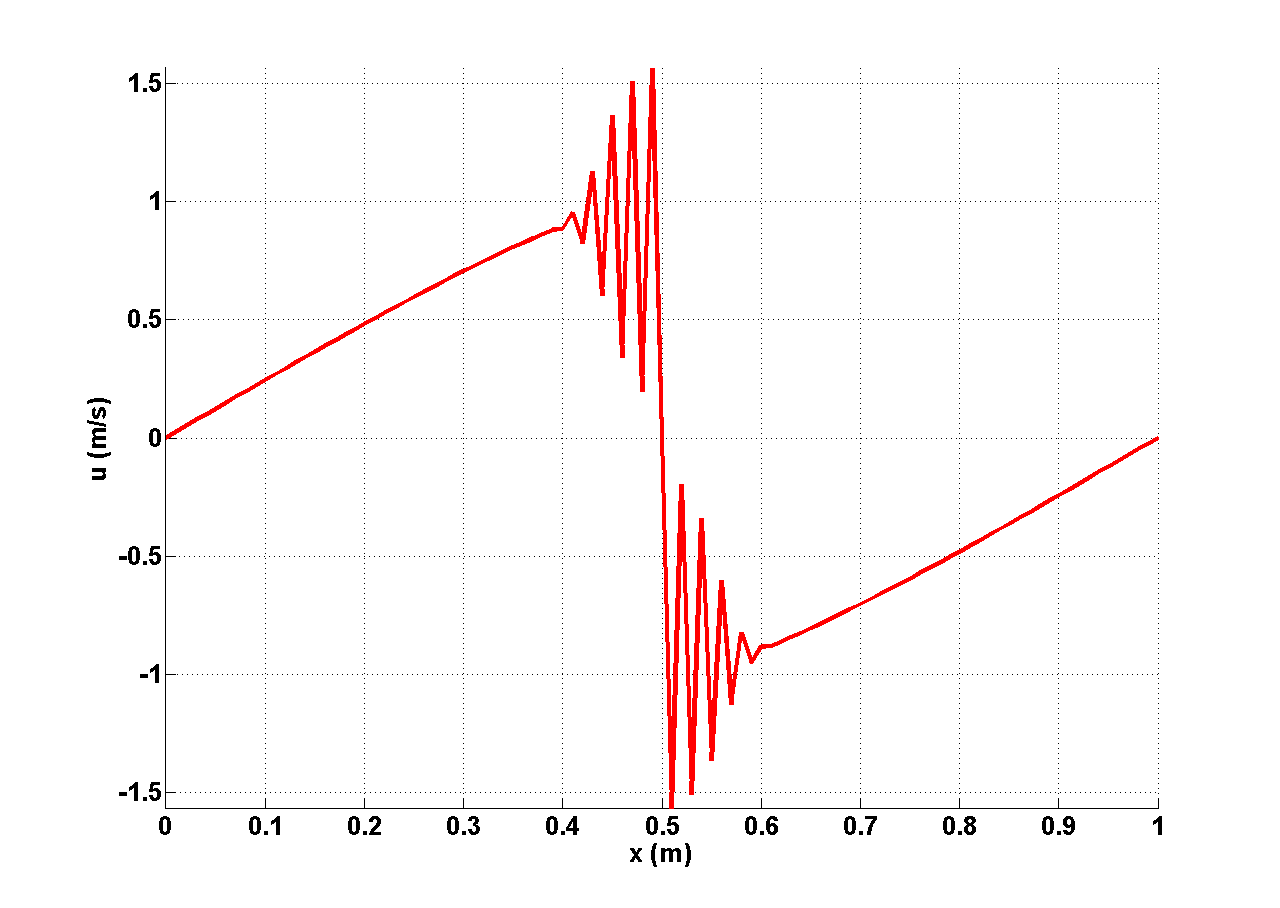
\includegraphics[width=\textwidth]{figs/1D_sol_free.png}
                \caption{Without stabilization.}
        \end{subfigure}%
        \begin{subfigure}[b]{0.37\textwidth}
                \centering
                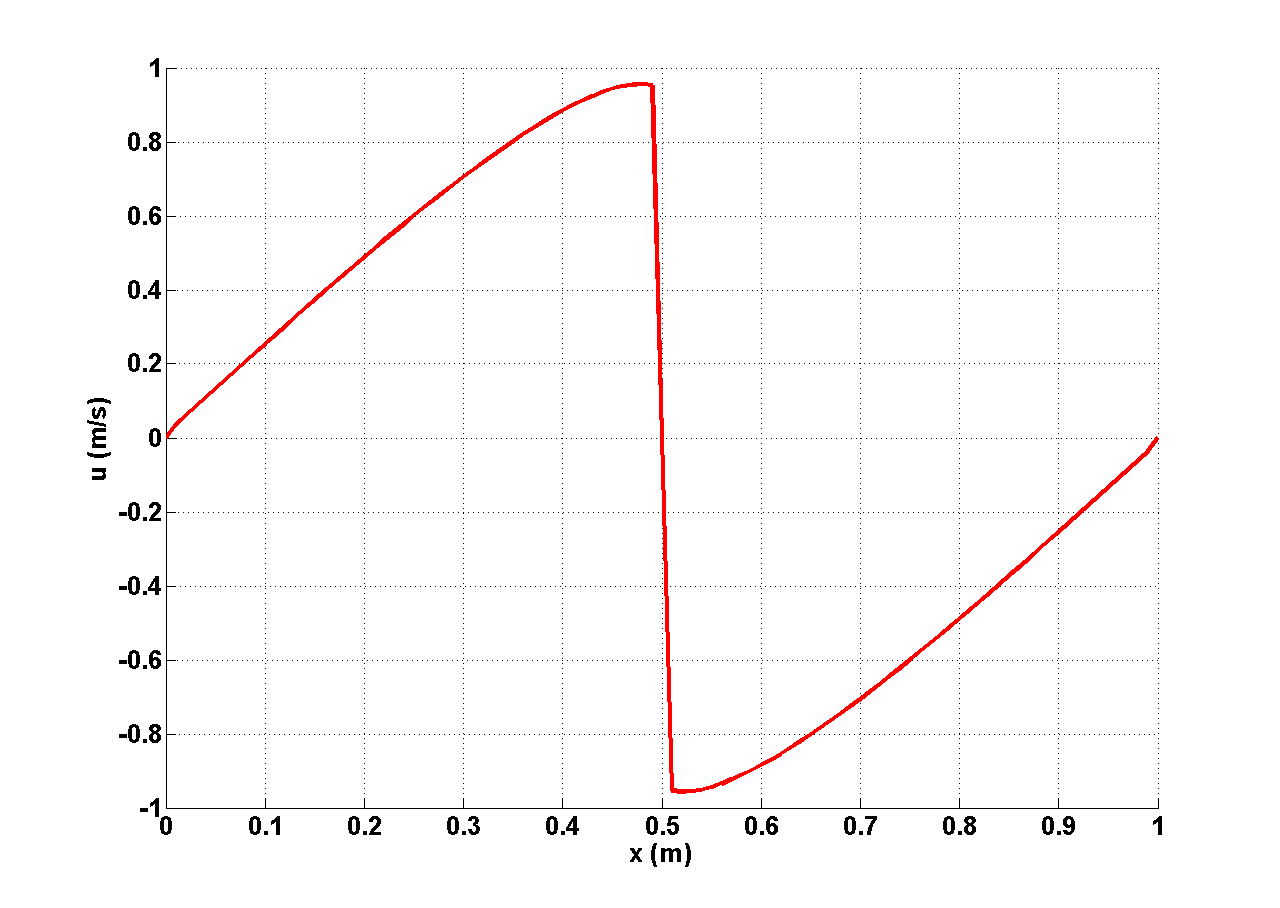
\includegraphics[width=\textwidth]{figs/1D_sol_fo.png}
                \caption{With first-order viscosity.}
        \end{subfigure}
        
        \begin{subfigure}[b]{0.37\textwidth}
                \centering
                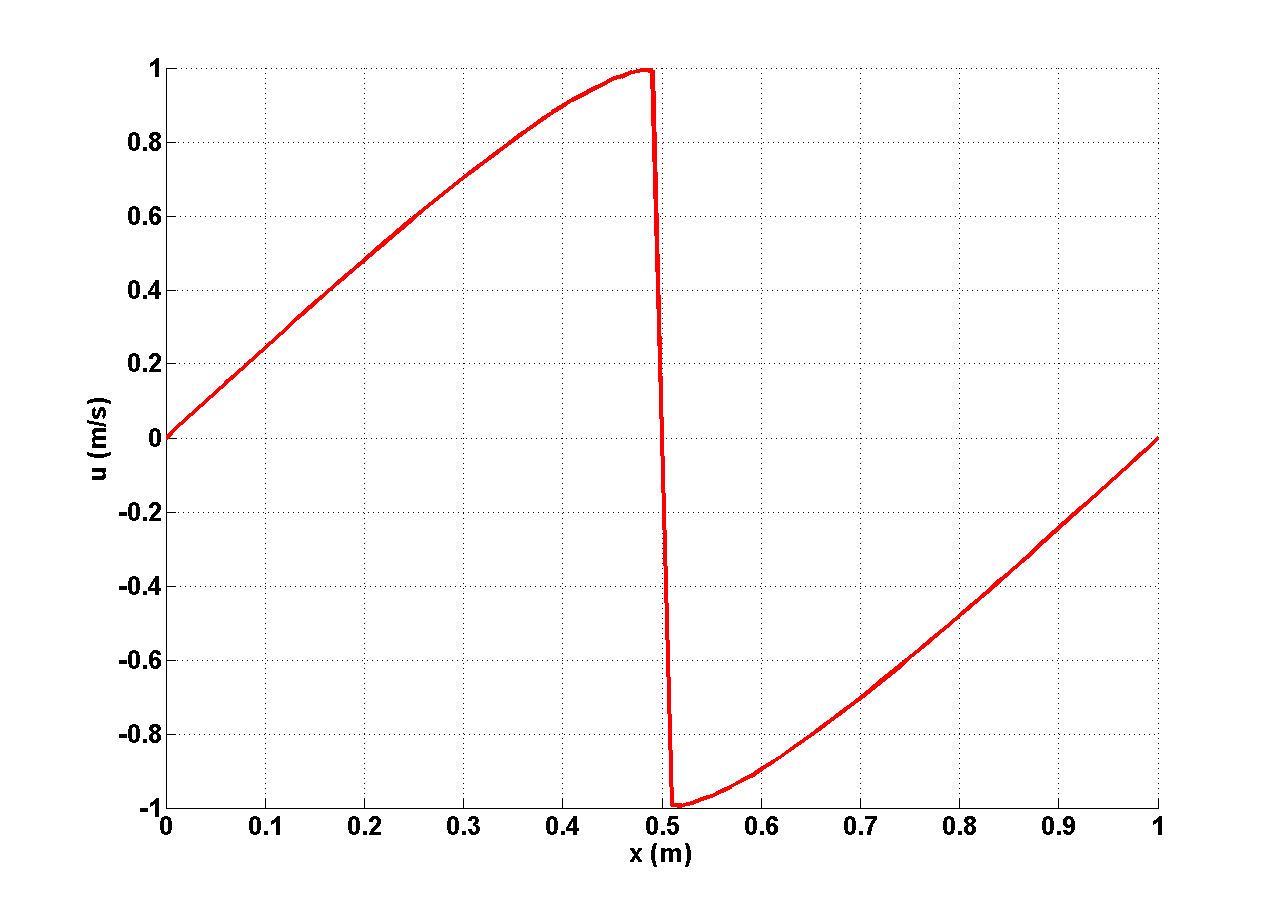
\includegraphics[width=\textwidth]{figs/1D_sol_ev.png}
                \caption{With the EVM.}
        \end{subfigure}
        \begin{subfigure}[b]{0.37\textwidth}
                \centering
                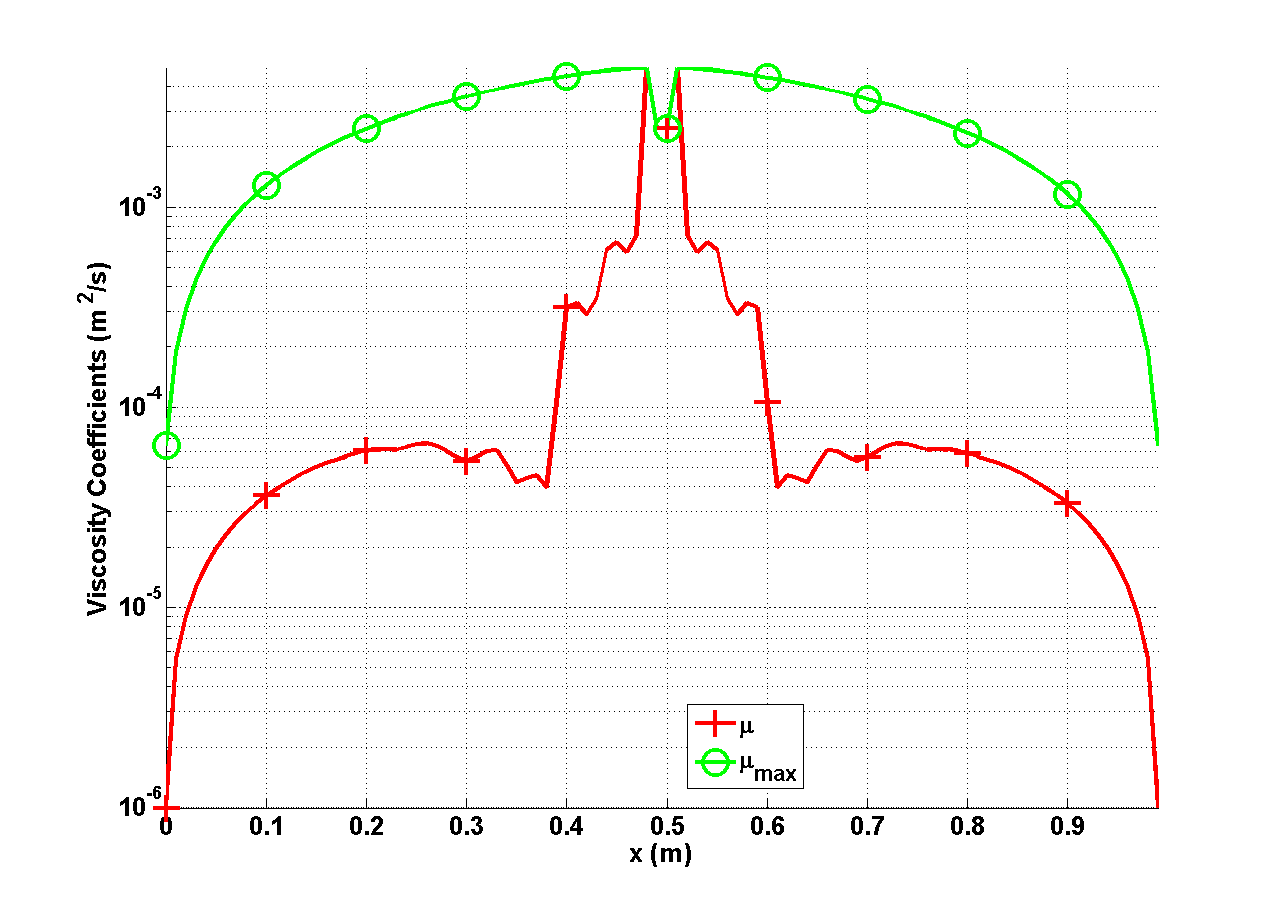
\includegraphics[width=\textwidth]{figs/1D_visc.png}
                \caption{Viscosity coefficient profiles.}
        \end{subfigure}
\end{figure}
\end{frame}
%************************************************************************************
\begin{frame}[shrink]{\normalsize A viscous regularization for the Seven-Equation two-phase flow Model}
\begin{block}{}
\begin{subequations}
%\left\{
%\begin{array}{lcll}
Void fraction equation: \\[-4pt]
\begin{equation}
\partial_t \left( \alpha_k  A\right) + A {\color{violet}\vec{u}_{int}} \cdot \grad \alpha_k = {\color{red}\mu_{rel}} {\color{blue}A \left( P_k - P_j \right)} + {\color{cyan}\div \left( A \beta_k \grad \alpha_k \right)}\nonumber 
\end{equation}
Continuity equation: \\[-4pt]
\begin{equation}
\partial_t \left( \alpha_k \rho_k A \right) + \div \left( \alpha_k \rho_k \vec{u}_k A \right) = {\color{cyan}\div \vec{f}} = {\color{cyan}\div \left[ A \left( \alpha_k \kappa_k \grad \rho_k + \rho_k \beta_k \grad \alpha_k \right) \right]} \nonumber
\end{equation}
Momentum equation: \\[-4pt]
\begin{align}
\partial_t \left( \alpha_k \rho_k \vec{u}_k A \right) + \div \left[ \alpha_k A \left( \rho_k \vec{u}_k\otimes \vec{u}_k \right) \right]  + \grad(\alpha_k A P_k) &=  \nonumber \\
\alpha_k P_k \grad A +  {\color{violet}P_{int}} A \grad \alpha_k +  {\color{red}\lambda_{rel}}{\color{blue}A  \left( \vec{u}_j - \vec{u}_k \right)} &+ {\color{cyan}\div \left[ A \alpha_k \rho_k \mu_k \grad^s \vec{u} + \vec{u} \otimes \vec{f} \right]}\nonumber
\end{align}
Energy equation:
\begin{align}
\partial_t \left( \alpha_k \rho_k E_k A \right) +& \div \left[ \alpha_k A \vec{u}_j \left( \rho_k E_k + P_k \right) \right] = \nonumber \\
&A {\color{violet}P_{int} \vec{u}_{int}} \cdot \grad \alpha_k - {\color{red}\mu_{rel}} {\color{violet}\bar{P}_{int}} {\color{blue}A\left( P_k-P_j \right)} + {\color{red}\lambda_{rel}} {\color{violet}\bar{\vec{u}}_{int}} {\color{blue}A \cdot \left( \vec{u}_j - \vec{u}_k \right)} +\nonumber \\
& {\color{cyan}\div \left[ A \alpha_k \kappa_k \grad (\rho e)_k - \frac{|| \vec{u}_k ||^2}{2} \vec{f} + A \alpha_k \mu_k \vec{u}_k : \grad^s \vec{u}_k \right]} \nonumber
\end{align}
%\end{array}
%\right.
\end{subequations}
\end{block}
\end{frame}
%************************************************
\begin{frame}[shrink]{\normalsize An all-Mach flow definition of the viscosity coefficients}
\begin{block}{\normalsize $\mu_k(\vec{r},t)    = \min \Big (\mu_{k,\max}(\vec{r},t), \mu_{k,e} (\vec{r},t)    \Big)$, and $\kappa_k(\vec{r},t) = \min \Big (\mu_{k,\max}(\vec{r},t), \kappa_{k,e} (\vec{r},t) \Big )$} 
\hspace{0.5cm} $\bullet$ $\ \kappa_{k,\max}(\vec{r},t)  = \mu_{k,\max} (\vec{r},t) = \frac{h}{2} \Big ( ||\vec{u}_k|| + c_k \Big )$.  \\ [3pt]
%
\hspace{0.5cm} $\bullet$ $\kappa_{k,e}(\vec{r},t) = \frac{h^2 \max(\resinew_k, J_k)}{ \textcolor{blue}{\rho_k c_k^2} }$ and
$\mu_{k,e}(\vec{r},t)    = \frac{h^2 \max(\resinew_k, J_k)}{ \textcolor{red}{\norm_{k,P}^\mu}}$  \\ [3pt]
%
\hspace{0.5cm} $\bullet$ $\resinew_k= \frac{DP_k}{Dt} - c_k^2 \frac{D\rho_k}{Dt}$ and $J_k = ||\vec{u_k} || \max \left( [[\ \grad P_k \cdot \vec{n}\ ]]  ,\ [[c_k^2 \grad \rho_k \cdot \vec{n} \ ]]\right)$ \\[3pt]
%
\hspace{0.5cm} $\bullet$ $\textcolor{red}{\norm_{k,P}^\mu} = \mathbb{G}(M_k) \rho_k || \vec{u}_k ||^2 + (1-\mathbb{G}(M_k)) \rho_k c_k^2$ and $\lim_{M_k \to 0} \mathbb{G}(M_k) = 0$ \\ [4pt]
%
\hspace{0.5cm} $\bullet$ $\mathbb{G}(M_k) = \frac{\tanh (a(M_k-M_\infty)) + |\tanh (a(M_k-M_\infty))|}{2}$
\end{block}
%
\begin{block}{\normalsize $\beta_k(\vec{r},t) = \min \Big (\beta_{k,\max}(\vec{r},t), \beta_{k,e} (\vec{r},t) \Big )$}
\hspace{0.5cm} $\bullet$ $\beta_{max} = \frac{h}{2} || \vec{u}_{int} ||$ and $\beta_{k,e} = h^2 \frac{\max( R_{k,\alpha}, J_{k,\alpha} )}{|| \eta_k - \bar{\eta}_k ||_\infty}$  \\ [3pt]
\hspace{0.5cm} $\bullet$ $R_{k,\alpha} = \partial_t \eta_k + \vec{u}_{int}\cdot \grad \eta_k$ with $\eta_k = \frac{\alpha_k^2}{2}$ and $J_{k,\alpha} = ||\vec{u}_{int} || \  [[\ \grad \alpha_k \cdot \vec{n}\ ]]$
\end{block}
\end{frame}
%************************************************
%\subsection{RELAP-7: reactor safety analysis code.}
%\begin{frame}{RELAP-7: reactor safety analysis code.}
%\begin{block}{What is RELAP-7?}
%\begin{itemize}
%\setlength{\itemsep}{15pt}
%\item Developed by Idaho National Laboratory (INL). 
%\item $1$-D reactor analysis system.
%\item Based on the MOOSE \cite{Moose} framework (C++): fully implicit code.
%\item Safety applications for PWR, BWR and gas reactors.
%\item Solve compressible system of equations using conservative variables $(\rho, \rho \vec{u}, \rho E)$.
%\end{itemize}
%\end{block}
%\end{frame}
%************************************************
\section{1-D numerical results}
%************************************************
\begin{frame}{}
\begin{block}{\normalsize Spatial and temporal discretizations}
\hspace{0.5cm} $\bullet$ BDF2 and linear polynomial test function \\
\hspace{0.5cm} $\bullet$ Ideal gas equation of states: $\gamma_1=1.4$ and $\gamma_2=3$ \\
\hspace{0.5cm} $\bullet$ 1-D pipe
\end{block}
%
\vspace{1cm}
Two tests for two limit cases:
\begin{block}{First test: two independent fluids}
\hspace{0.5cm} $\bullet$ Both fluids initially at rest, ($P_{left} = $,  $P_{right} = $) and ($T_{left} = $, $T_{right} = $) \\
\hspace{0.5cm} $\bullet$ Zero relaxation coefficients: $\mu_rel = \lambda_{rel} = 0$
\end{block}
%
\begin{block}{Second test: infinite relaxation parameters (Kapila)}
\hspace{0.5cm} $\bullet$ Same initial conditions \\
\hspace{0.5cm} $\bullet$ Zero relaxation coefficients: $\mu_{rel} = \lambda_{rel} = \infty$
\end{block}
\end{frame}
%************************************************
\begin{frame}[shrink]{$1$-D shock tube with two independent fluids}
\begin{figure}
        \begin{subfigure}[h]{\textwidth}
                \centering
                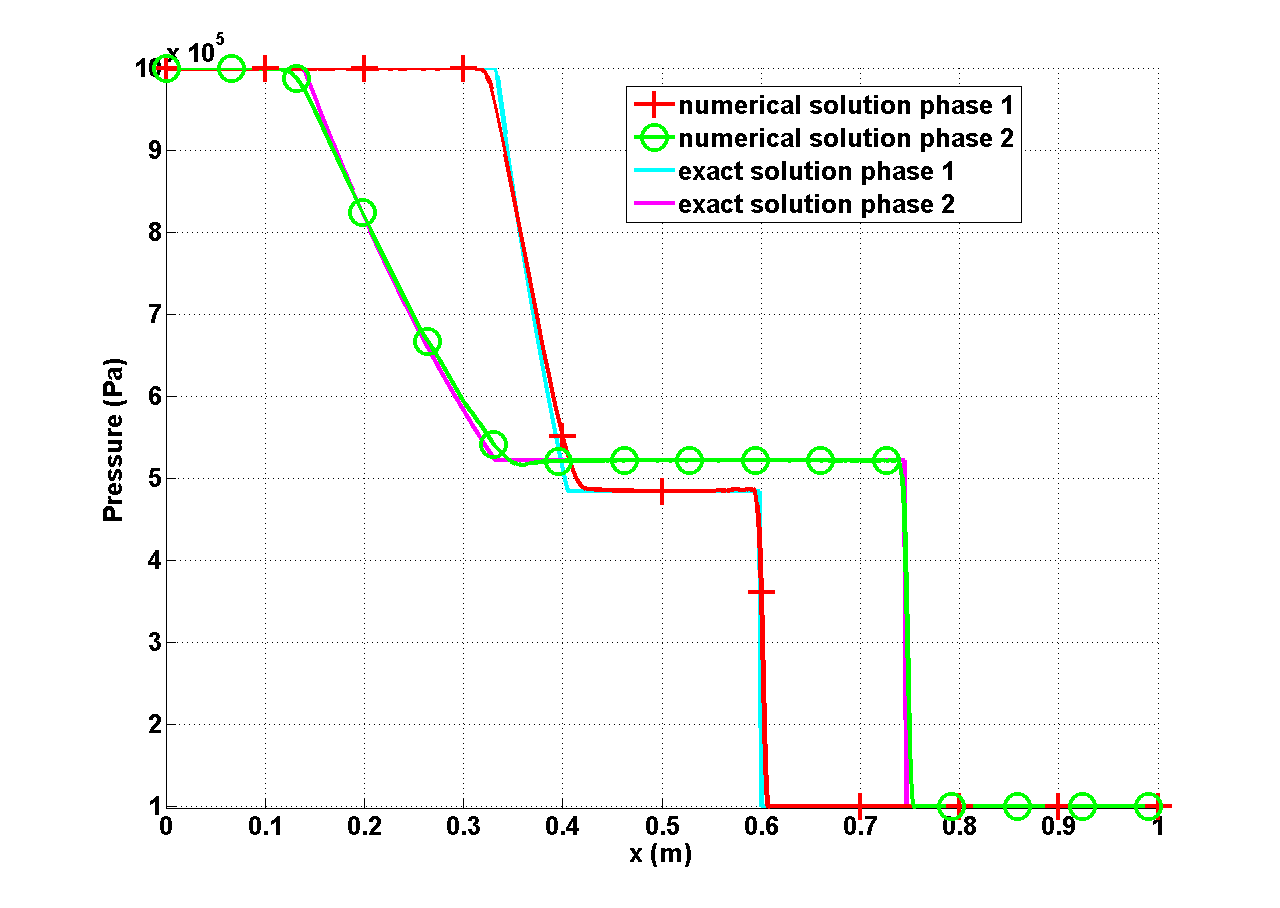
\includegraphics[width=\textwidth]{figs/two_phases_pressure.png}
                \caption{\huge Pressure at $t=305$ $\mu s$}
        \end{subfigure}%
        \begin{subfigure}[h]{\textwidth}
                \centering
                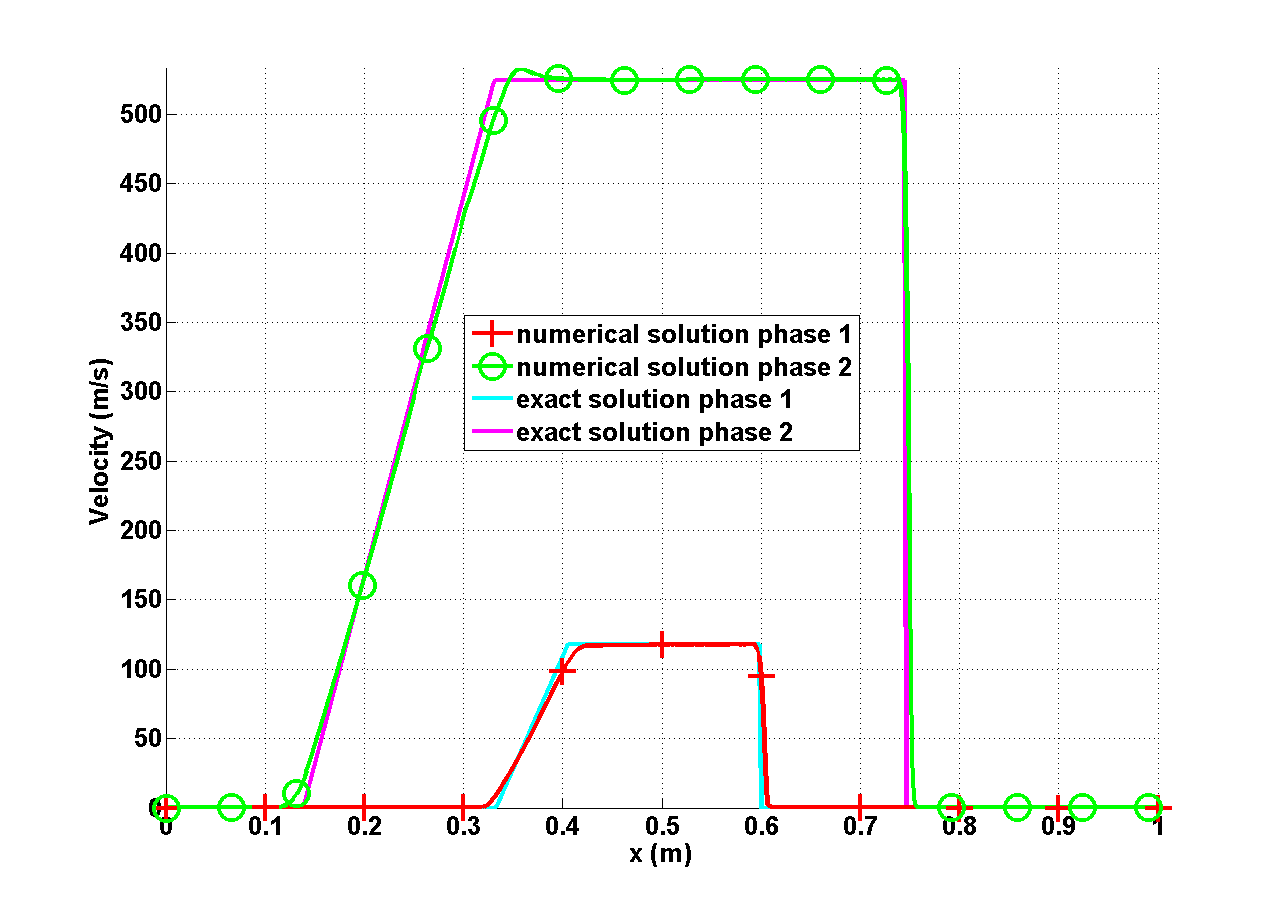
\includegraphics[width=\textwidth]{figs/two_phases_velocity.png}
                \caption{\huge Velocity at $t=305$ $\mu s$}
        \end{subfigure}%

        \begin{subfigure}[h]{\textwidth}
                \centering
                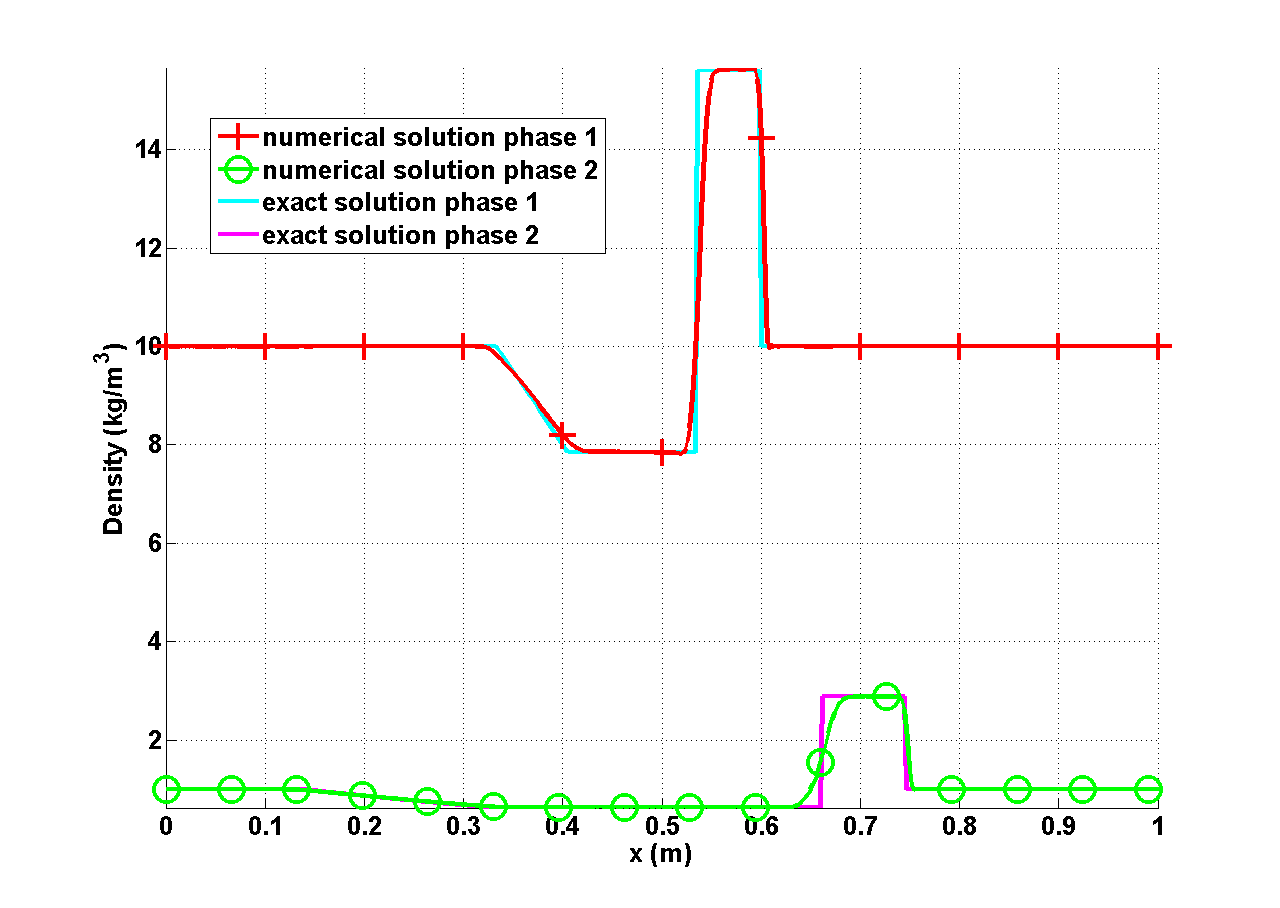
\includegraphics[width=\textwidth]{figs/two_phases_density.png}
                \caption{\huge Density at $t=305$ $\mu s$}
        \end{subfigure}%
        \begin{subfigure}[h]{\textwidth}
                \centering
                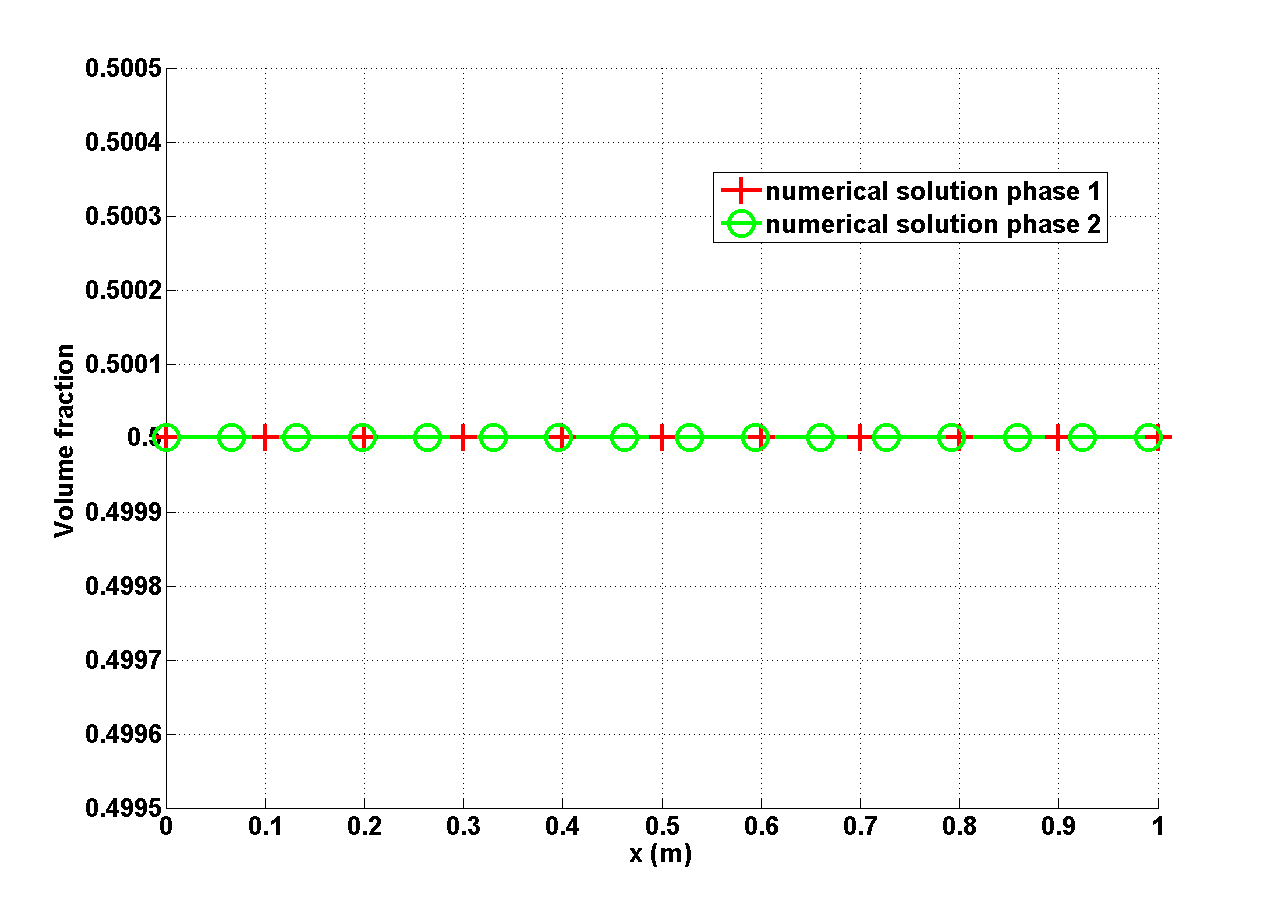
\includegraphics[width=\textwidth]{figs/two_phases_volume_fraction.png}
                \caption{\huge Volume fraction at $t=305$ $\mu s$}
        \end{subfigure}%
\end{figure}
\end{frame}
%************************************************
\begin{frame}[shrink]{$1$-D shock tube with two independent fluids}
\begin{figure}
        \begin{subfigure}[b]{\textwidth}
                \centering
                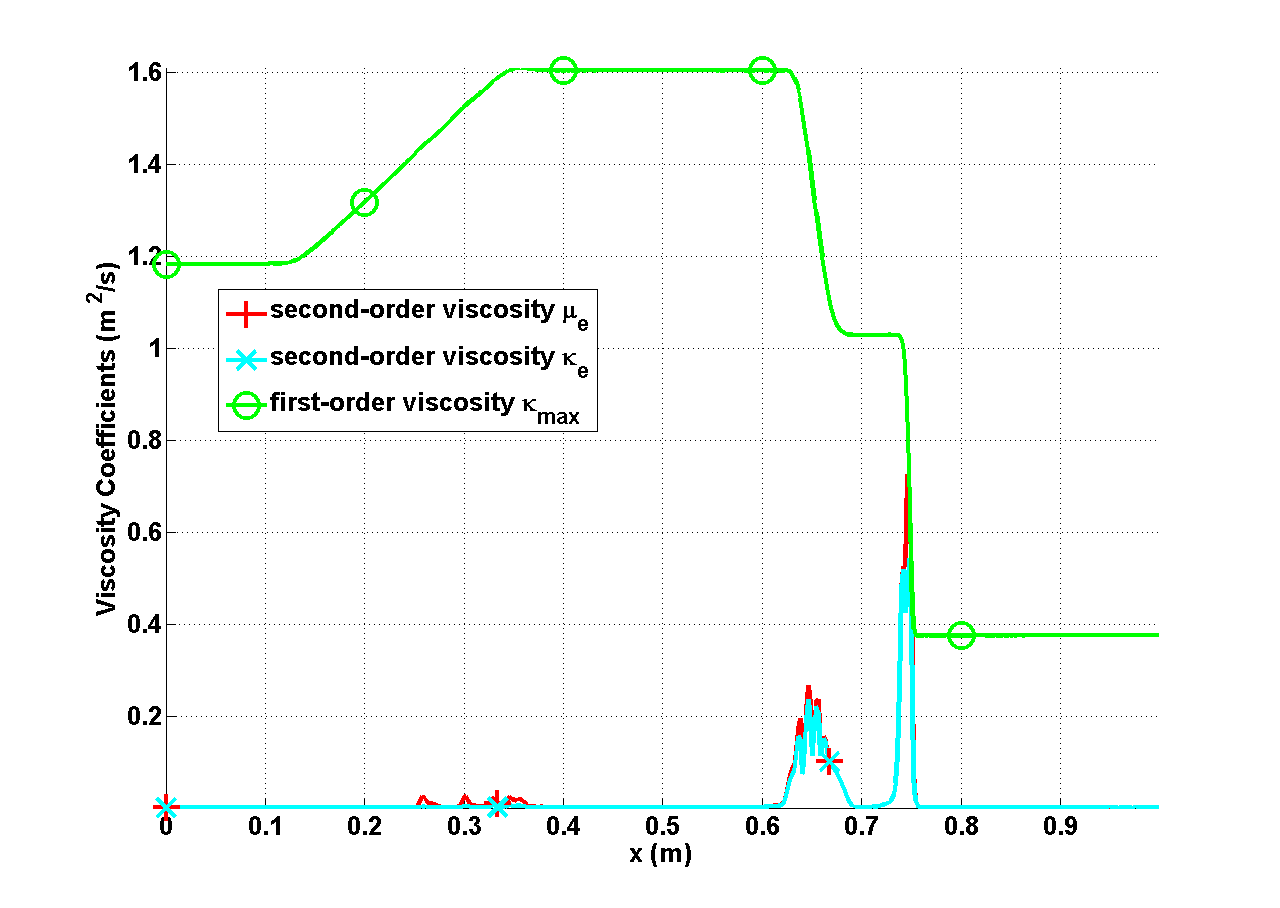
\includegraphics[width=\textwidth]{figs/two_phases_liquid_viscosity_kappa_mu.png}
                \caption{\huge Viscosity coefficients phase $1$}
        \end{subfigure}%
        \begin{subfigure}[b]{\textwidth}
                \centering
                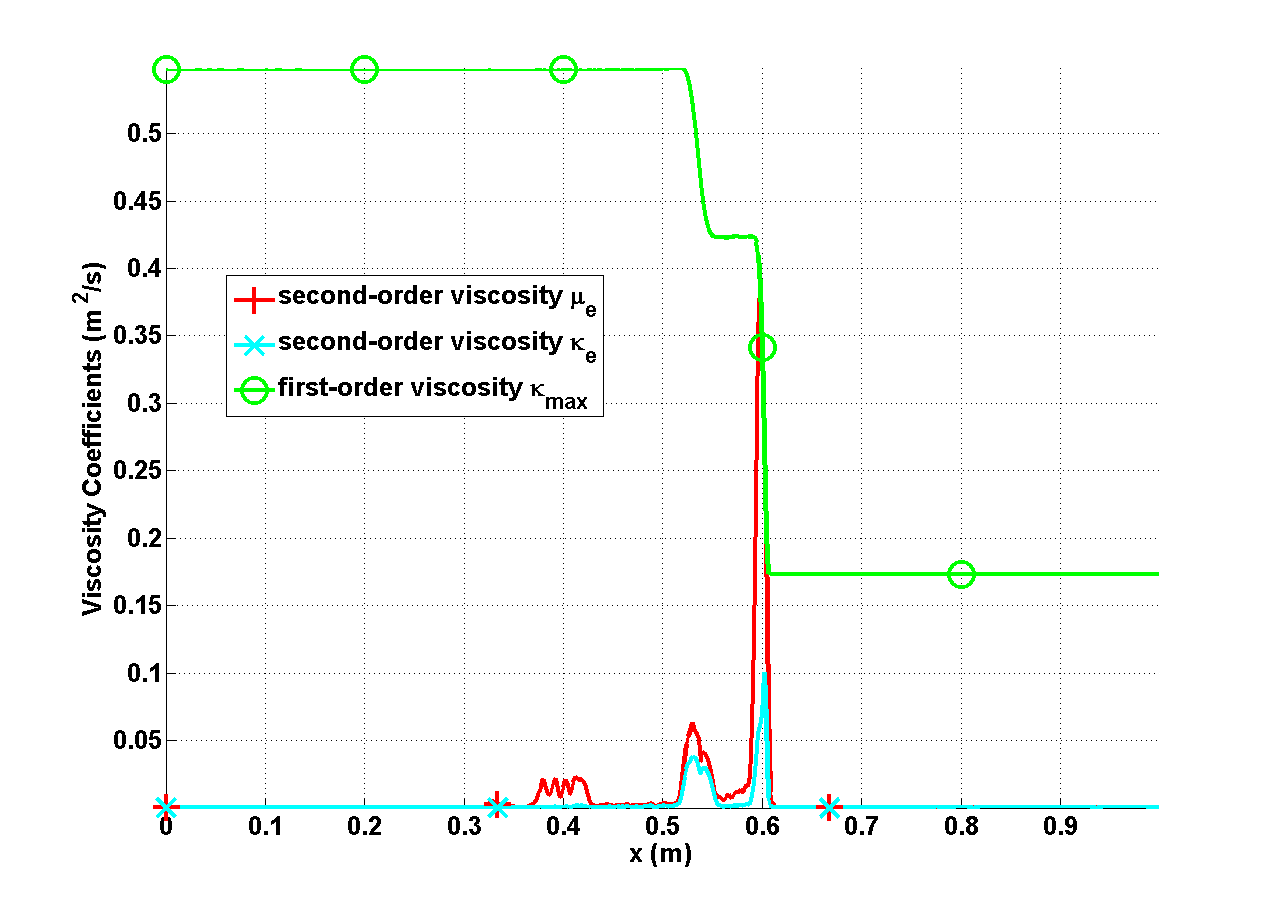
\includegraphics[width=\textwidth]{figs/two_phases_vapor_viscosity_kappa_mu.png}
                \caption{\huge Viscosity coefficients phase $2$}
        \end{subfigure}%
\end{figure}
\begin{figure}[H]        
\centering
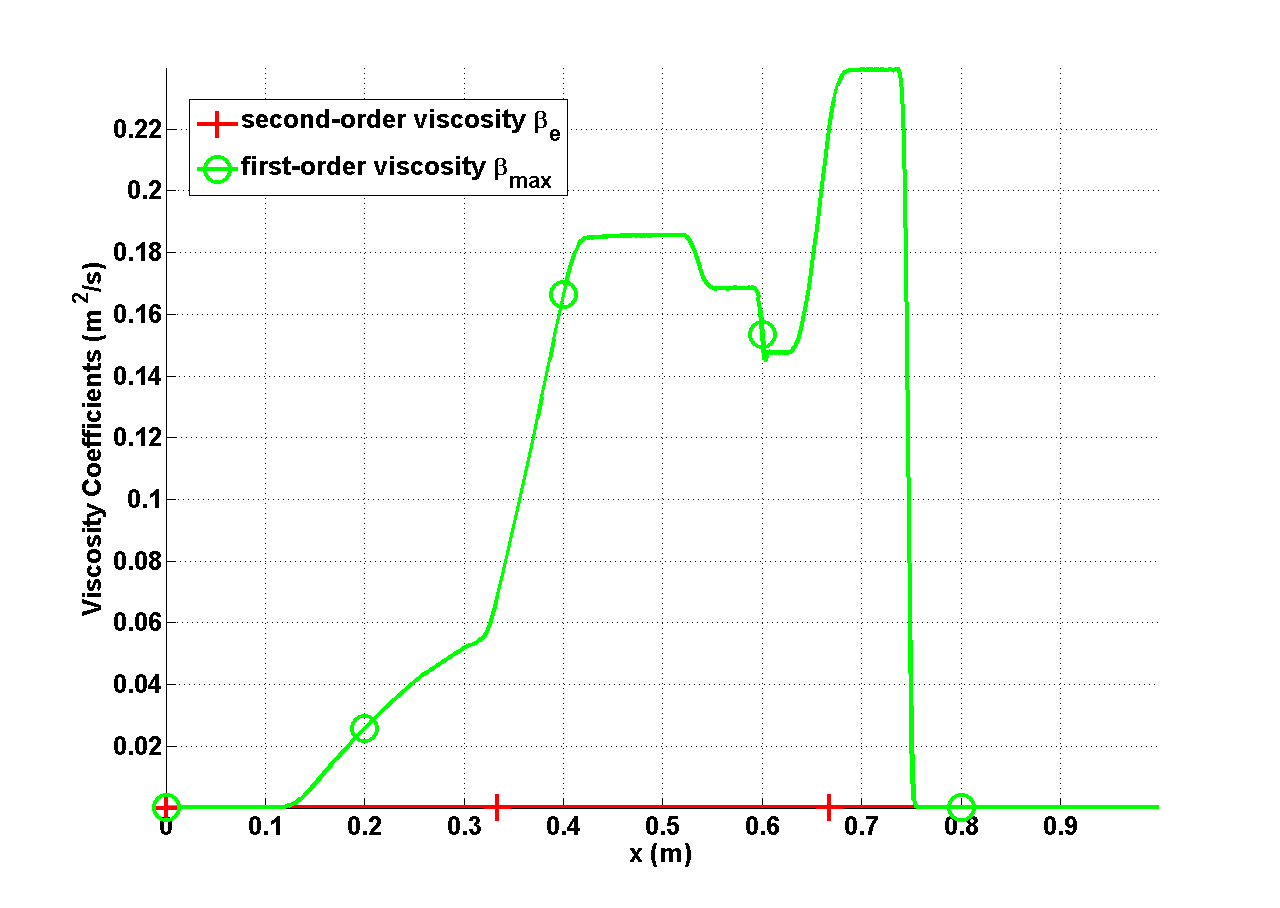
\includegraphics[width=\textwidth]{figs/two_phases_liquid_beta.png}
\caption{\huge Viscosity coefficients volume fraction}
\end{figure}
\end{frame}
%************************************************
\begin{frame}[shrink]{\normalsize $1$-D shock tube with infinite relaxation coefficients}
\begin{figure}
        \begin{subfigure}[b]{\textwidth}
                \centering
                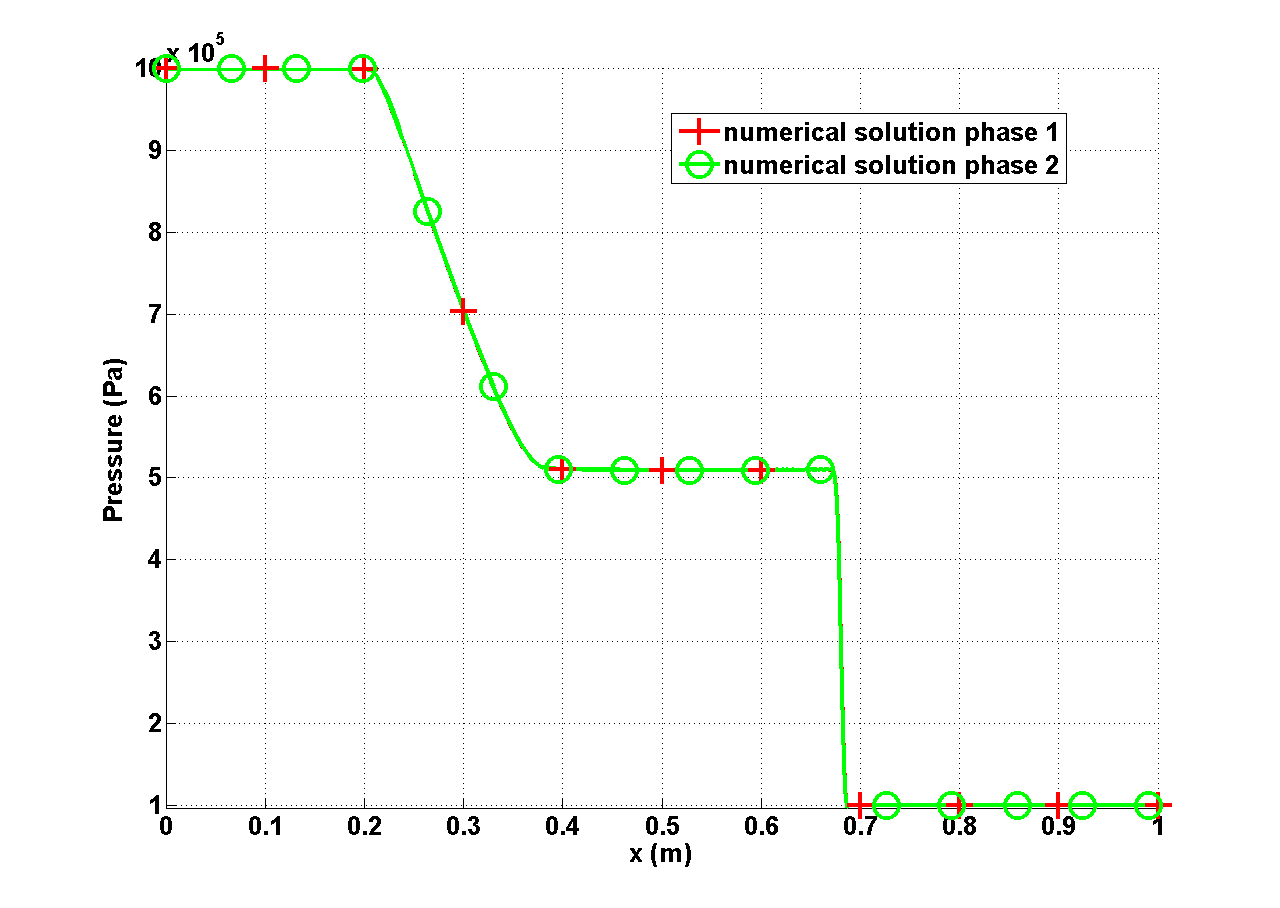
\includegraphics[width=\textwidth]{figs/relaxation_two_phases_pressure.png}
                \caption{\huge Pressure at $t=305$ $\mu s$}
        \end{subfigure}%
        \begin{subfigure}[b]{\textwidth}
                \centering
                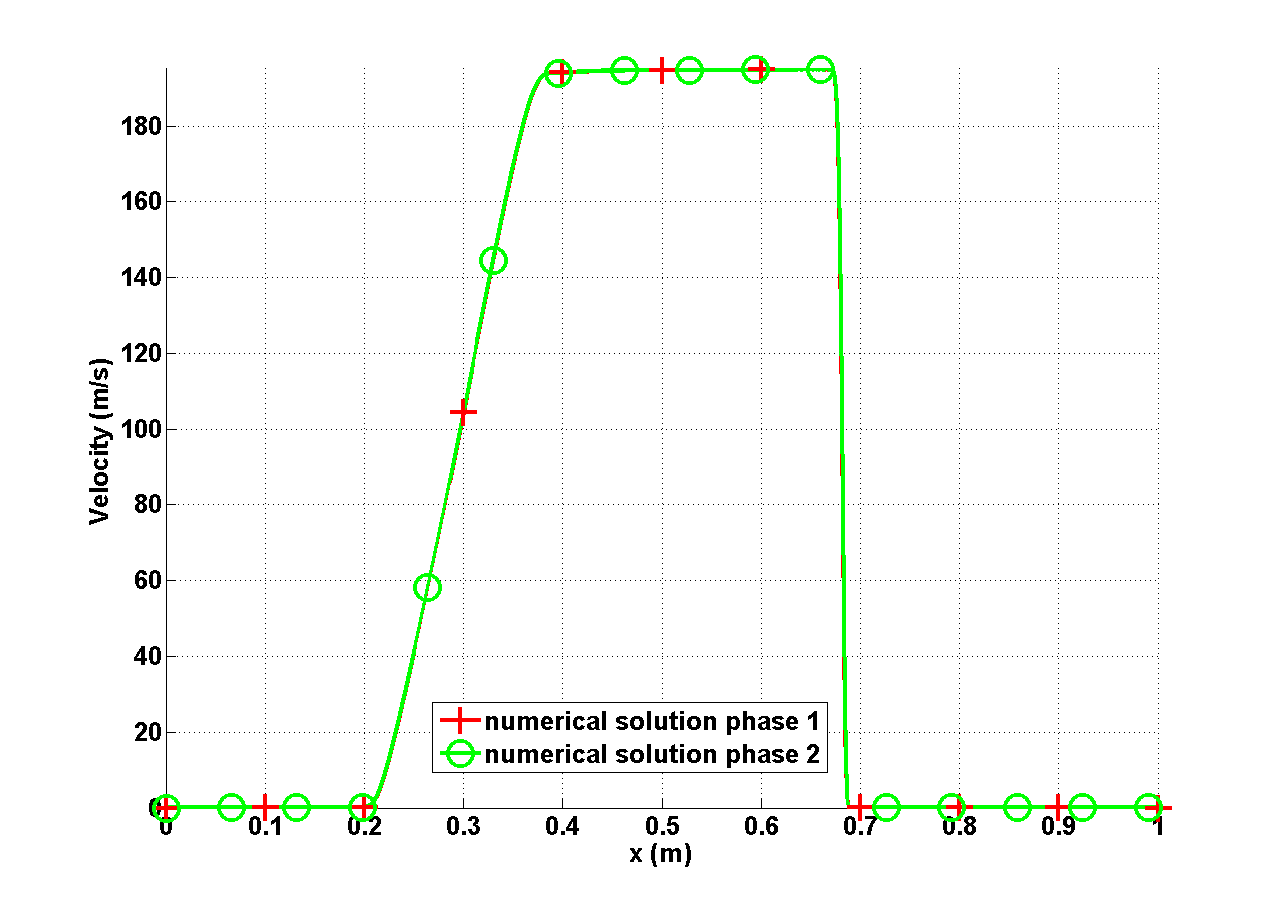
\includegraphics[width=\textwidth]{figs/relaxation_two_phases_velocity.png}
                \caption{\huge Velocity at $t=305$ $\mu s$}
        \end{subfigure}%

        \begin{subfigure}[b]{\textwidth}
                \centering
                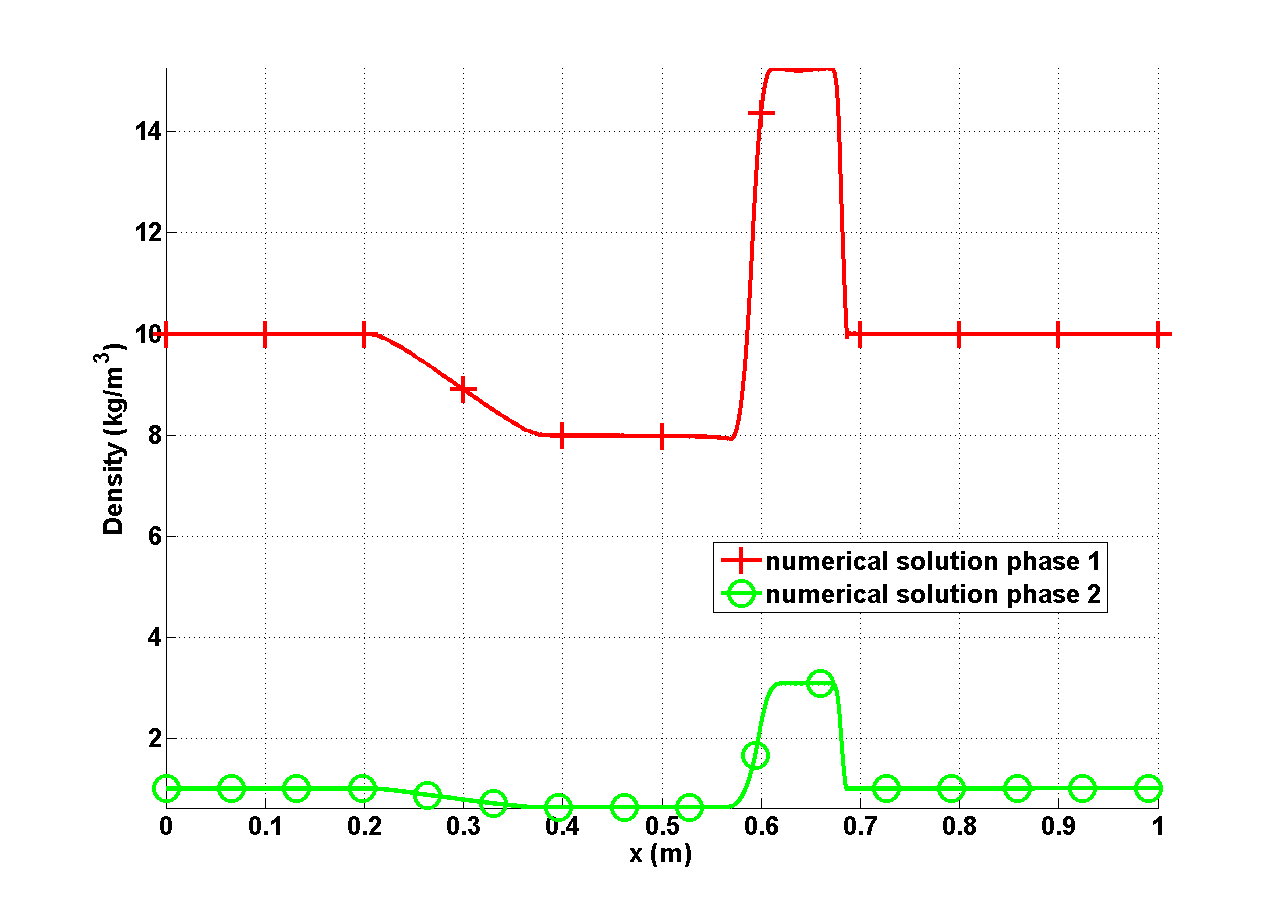
\includegraphics[width=\textwidth]{figs/relaxation_two_phases_density.png}
                \caption{\huge Density at $t=305$ $\mu s$}
        \end{subfigure}%
        \begin{subfigure}[b]{\textwidth}
                \centering
                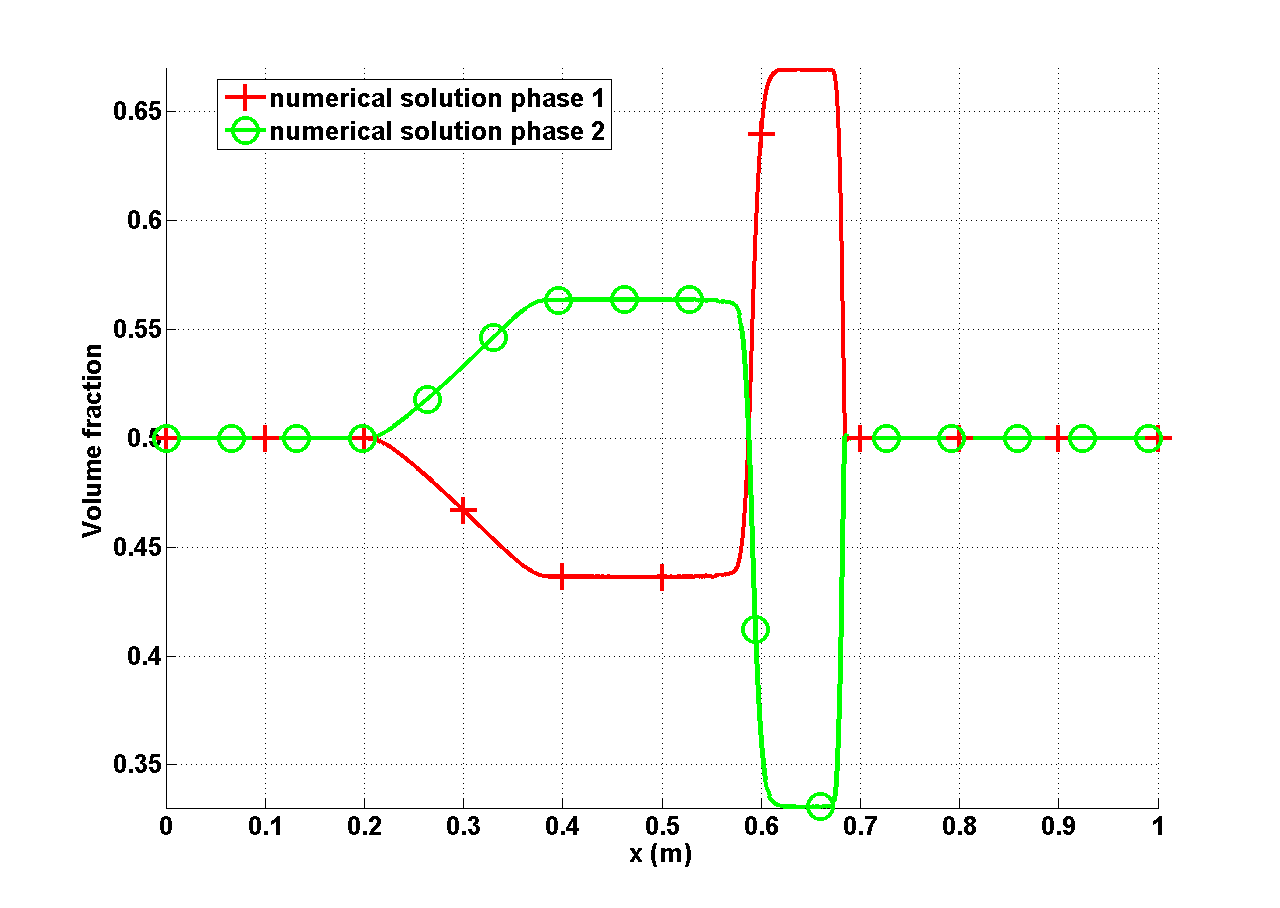
\includegraphics[width=\textwidth]{figs/relaxation_two_phases_volume_fraction.png}
                \caption{\huge Volume fraction at $t=305$ $\mu s$}
        \end{subfigure}%
\end{figure}
\end{frame}
%************************************************
\begin{frame}[shrink]{\normalsize $1$-D shock tube with infinite relaxation coefficients}
\begin{figure}
        \begin{subfigure}[b]{\textwidth}
                \centering
                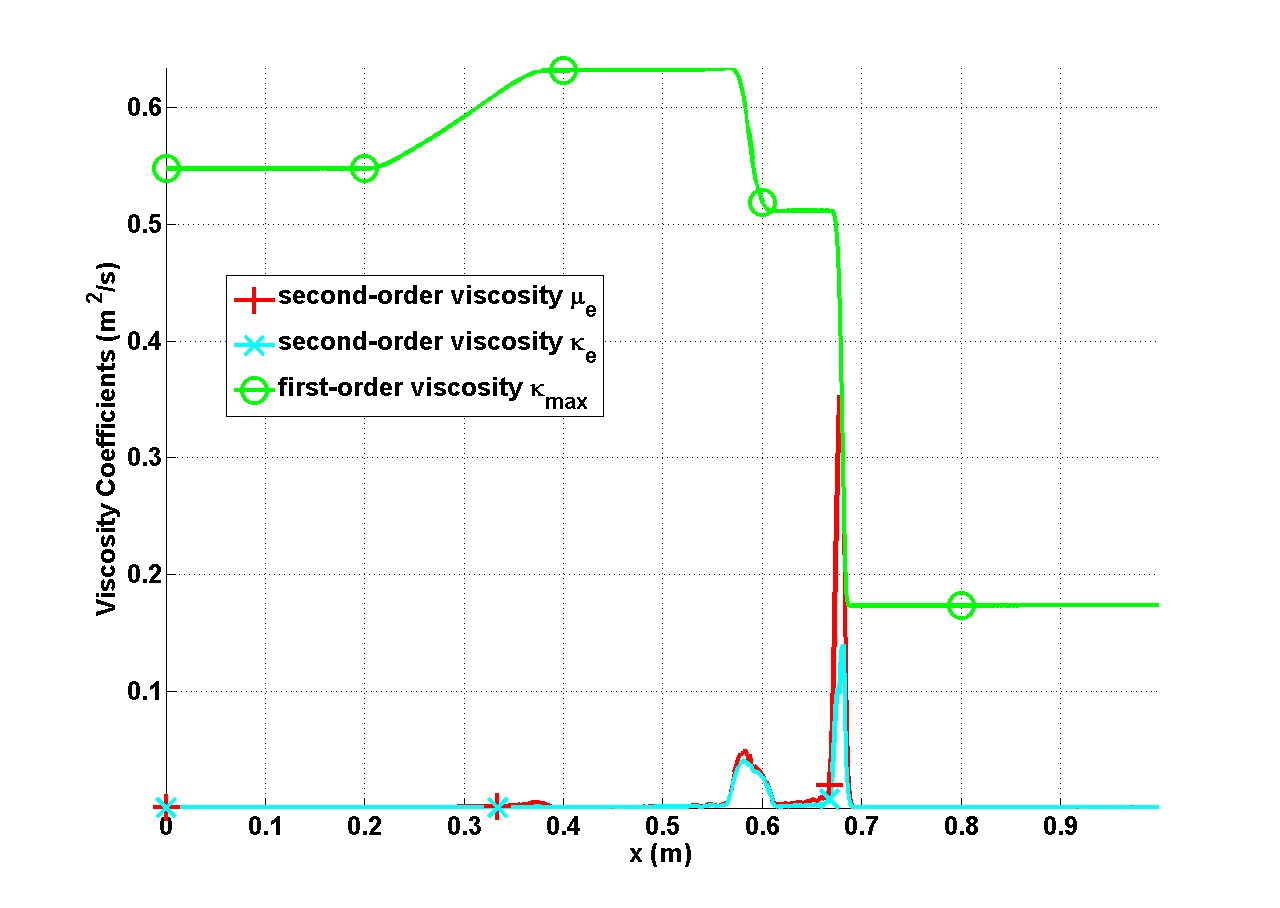
\includegraphics[width=\textwidth]{figs/relaxation_two_phases_liquid_viscosity_kappa_mu.png}
                \caption{\huge Viscosity coefficients phase $1$}
        \end{subfigure}%
        \begin{subfigure}[b]{\textwidth}
                \centering
                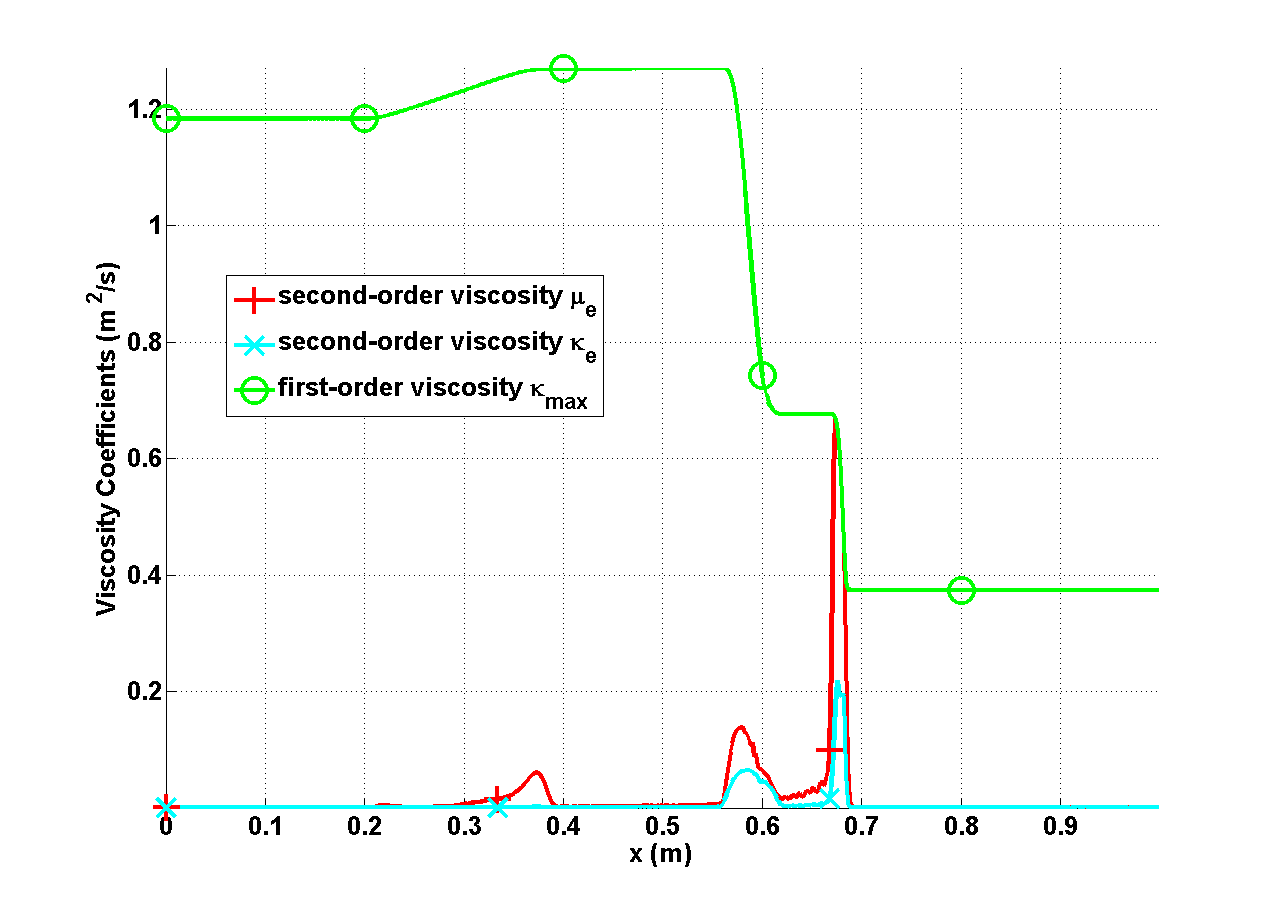
\includegraphics[width=\textwidth]{figs/relaxation_two_phases_vapor_viscosity_kappa_mu.png}
                \caption{\huge Viscosity coefficients phase $2$}
        \end{subfigure}%
\end{figure}
\begin{center}
\begin{figure}[!h] 
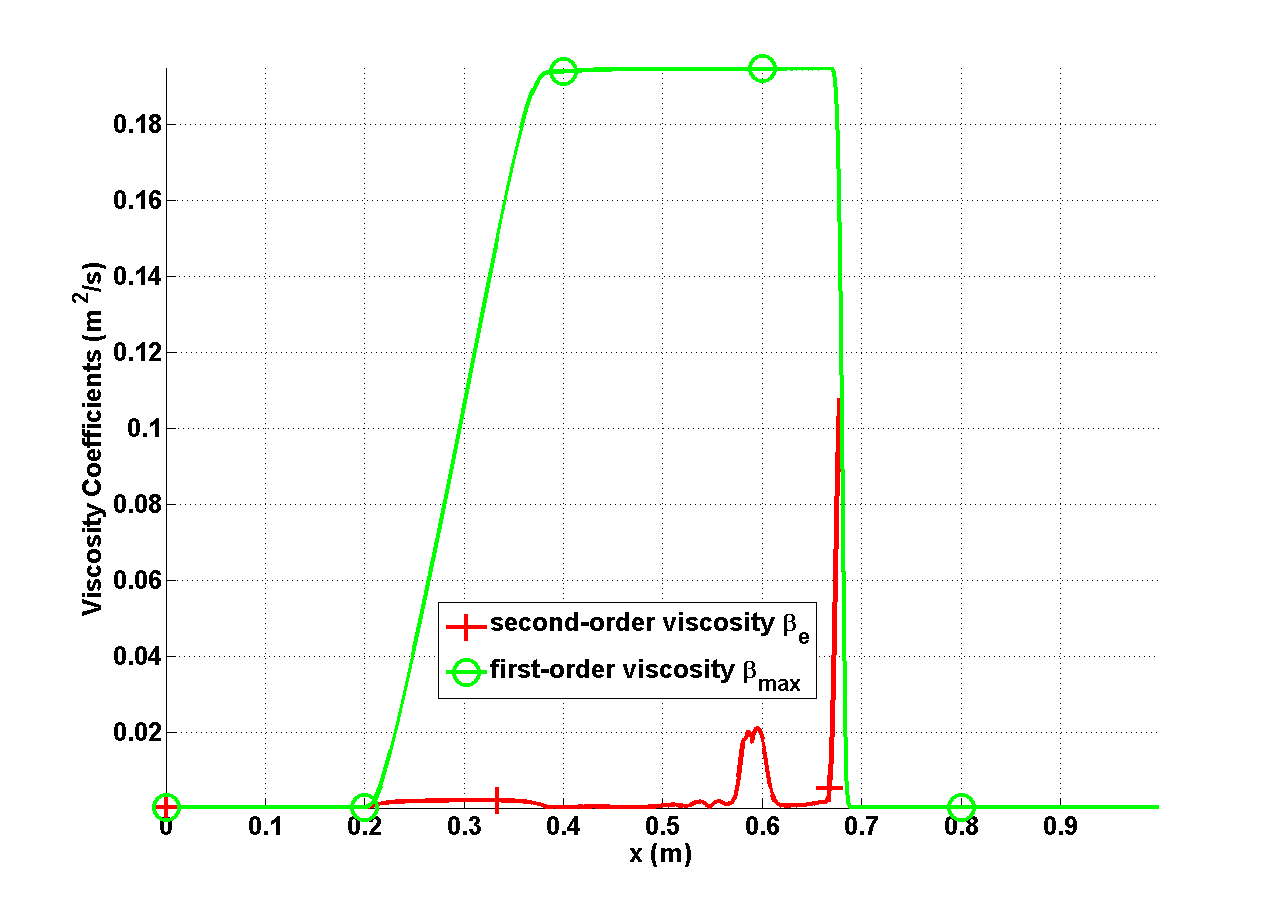
\includegraphics[width=\textwidth]{figs/relaxation_two_phases_liquid_beta.png}
\caption{\huge Viscosity coefficients volume fraction}
\end{figure}
\end{center}
\end{frame}
%************************************************
\section{Conclusions and future work}
\begin{frame}[shrink]{\normalsize Conclusions and future work}
\begin{block}{Conclusions}
\hspace{0.5cm} $\bullet$ Derived a viscous regularization for the SEM that is consistent with the entropy minimum principle \\
\hspace{0.5cm} $\bullet$ All-Mach flow definition of the viscosity coefficients \\
\hspace{0.5cm} $\bullet$ Presented numerical results using a \emph{continuous} FEM spatial discretization and an implicit (BDF2) temporal integration \\
\hspace{0.5cm} $\bullet$ Method is a RELAP-7, a MOOSE-based application of the INL
\end{block}
\begin{block}{Future work}
\hspace{0.5cm} $\bullet$ Further 1-D tests: hydrostatic tests, stronger shocks \\
\hspace{0.5cm} $\bullet$ Multi-D simulations $\rightarrow$ requires a preconditioner \\
\hspace{0.5cm} $\bullet$ Implement the EVM using a discontinuous schemes for comparison against approximate Riemann solver
\end{block}
\end{frame}
%************************************************
\begin{frame}{}
\begin{center}
\LARGE{\textbf{QUESTIONS/COMMENTS ?}}
\end{center}
\end{frame}
%************************************************
%************************************************
%************************************************
%************************************************
%************************************************
%************************************************
%************************************************
%************************************************
%\bibliographystyle{ans}
%\bibliography{mybibfile}
\begin{frame}[allowframebreaks]
\bibliographystyle{apalike}
\bibliography{Biblio-Database}
\begin{thebibliography}{47}
  
%  \bibitem{jlg1}
%  {\em Entropy viscosity method for nonlinear conservation laws}, 
%  Jean-Luc Guermond, R. Pasquetti, B. Popov, J. Comput. Phys., 230 (2011) 4248-4267.
%  
%  \bibitem{jlg2}
%  {\em Entropy Viscosity Method for High-Order Approximations of Conservation Laws}, 
%  J-L. Guermond, R. Pasquetti, 
%  Lecture Notes in Computational Science and Engineering, Springer, Volume 76, (2011) 411-418.
%
% \bibitem{jlg3}
% \emph{Entropy-based nonlinear viscosity for Fourrier approximations of conservation laws}, 
% J.-L. Guermond, R. Pasquetti, C.R. Math. Acad. Sci. Paris 346 (2008) 801�806.
%
%  \bibitem{Neumann}
%  \emph{A method for the numerical calculation of hydrodynamic shocks}, 
%  J. von Neumann, R.D. Richtmyer, J. Appl. Phys. 21 (1950) 232�237
%  
%  \bibitem{Balsara}
%  \emph{An Analysis of the Hyperbolic Nature of the Equations of Radiation Hydrodynamics},
%  Dinshaw S. Balsara, J. Quant. Spectrosc. Radiat. Transfer, Vol. 61, No. 5, pp. 617-627, 1999.
%  
%  \bibitem{LowrieMorelHittinger}
%  \emph{The coupling of radiation and hydrodynamics},
%  Lowrie RB, Morel JE, Hittinger JA, 521 (1), 432-50 (1999).
%
%  \bibitem{FluxLimiter1}
%  \emph{Advanced numerical approximation of nonlinear hyperbolic equations}, 
%  B. Cockburn, C. Johnson, C. Shu, E. Tadmor, Lecture Notes in Mathematics, vol. 1697, Springer, 1998.
%  
%  \bibitem{FluxLimiter2}
%  \emph{Discontinuous Galerkin methods: theory, computation and applications}, 
%  B. Cockburn, G. Karniadakis, C. Shu, Lecture Notes in Computer Science and Engineering, vol. 11, Springer, 2000.
%  
%  \bibitem{FluxLimiter3}
%  \emph{The local discontinuous Galerkin method for time- dependent convection-diffusion systems}, 
%  B. Cockburn, C. Shu, SIAM J. Numer. Anal. 35 (1998) 2440�2463.
%  
%\bibitem{FluxLimiter4}
%\emph{New non-oscillatory central schemes on unstructured triangulations for hyperbolic systems of conservation laws}, 
%I. Christov, B. Popov, J. Comput. Phys. 227 (11) (2008) 5736�5757.
%
%\bibitem{SUPG}
%\emph{Streamline upwind/Petrov-Galerkin formulations for convection dominated flows with particular emphasis on the incompressible Navier-Stokes equations},
%A.N. Brooks, T.J.R. Hughes, Comput. Meths. Appl. Mech. Engrg., 32 (1982), pp. 199�259.
%
%\bibitem{EdwardsMorelKnoll}
% \emph{Nonlinear variants of the TR$-$BDF$2$ method for thermal radiative diffusion},
% Jarrods D. Edwards, Jim E. Morel, Dana A. Knoll, Journal of Computational Physics, 230 (2011), 1198-1214.
% 
%  \bibitem{Toro}
%  \emph{Riemann Solvers and numerical methods for fluid dynamics.}
%  E.F. Toro, $2^{nd}$ Edition, Springer.  
%  
%  \bibitem{Reisner}
%  \emph{A space-time smooth artificial viscosity method for nonlinear conservation laws}
%  Reisner J., Serencsa J. and Shkoller S., Journal of Computational Physics 235 (2013) 912-933.
%    
%  \bibitem{valentin}
%  \emph{Implementation of the entropy viscosity method with the discontinuous Galerkin method},
%  Valentin Zingan, Jean-Luc Guermond, Jim Morel, Bojan Popov, Volume 253, 1 January 2013, Pages 479-490
%    
%  \bibitem{LowrieMorel}
%  \emph{Issues with high-resolution Godunov methods for radiation hydrodynamics},
%  R.B. Lowrie, J.E. Morel, Journal of Quantitative Spectroscopy \& Radiative Transfer, 69, 475-489 (2001).
%
%\bibitem{EdwardsMorelLowrie}
%\emph{Second-Order Discretization in Space and Time for Radiation Hydrodynamics},
%Jarrod D. Edwards, Jim E. Morel, Robert B. Lowrie, International Conference on Mathematics and Computational Methods Applied to Nuclear Science \& Engineering (M\&C 2013), Sun Valley, Idaho USA, May 5-9, American Nuclear Society, LaGrange Park, II (2013).
%   
%  \bibitem{ShiJin}
%  \emph{Numerical Schemes for Hyperbolic Conservation Laws with Stiff Relaxation Terms}, 
%  Shi Jin and C. David Levermore, Journal of Computational Physics, 126, 449-467 (1996).
%  
%  \bibitem{jlg}
%  \emph{Viscous regularization of the Euler equations and entropy principles},
%  Jean-Luc Guermond and Bojan Popov, under review.
%  
%  \bibitem{Moose}
%  \emph{A parallel computational framework for coupled systems of nonlinear equations},
%  D. Gaston, C. Newsman, G. Hansen and D. Lebrun-Grandie, Nucl. Eng. Design, vol 239, pp 1768-1778, 2009.
%  
%  \bibitem{Sodov}
%  \emph{Similarity and dimensional methods in mechanics},
%  Sedov LI., New York: Academic Press, 1959.
%  
%  \bibitem{RatTherm}
%  \emph{Rational thermodynamics},
%  Truesdell C. and Wang C.-C., New York, McGraw-Hill Book Company, 1969, XII. 208 S.
%  
%  \bibitem{IGEOS}
%  \emph{A to Z of Thermodynamics},
%  Perrot P., Oxford University Press (1998).
%  
%  \bibitem{SGEOS}
%  \emph{Elaborating equation of state for a liquid and its vapor for two-phase flow models.}
%  O. LeMetayer, J. Massoni, R. Saurel, International Journal of Thermal Science 43 (2004) 265-276.
%
%  \bibitem{Lapidus_paper}
%  \emph{A detached shock calculation by second order finite differences},
%  Lapidus A., J. Comput. Phys., 2, 154-177.
%
%  \bibitem{LMP}
%  \emph{A simple extension to multidimensional problems of the artificial viscosity due to Lapidus},
%  Lohner R., Morgan K. and Peraire J., Commun. Numer. Methods Eng., 1(14), 141-147.
%      
%  \bibitem{Lapidus_book}
%  \emph{Finite Element Methods for Flow Problems},
%  Jean Donea and Antonio Huerta, 2003,  Edition, Wiley.
%  
%  \bibitem{PBV_book}
%  \emph{Applied CFD Techniques: an Introduction based on Finite Element Methods},
%  Rainald Lohner, $2^{nd}$ Edition, Wiley.
%  
%  \bibitem{Roe}
%  \emph{An All-Speed Roe-type scheme and its asymptotic analysis of low Mach number behavior},
%  Xue-song Li, Chun-wei Gu, Journal of Computational Physics 227 (2008) 5144-5159
%  
%  \bibitem{LowMach1}
%  \emph{On the behavior of upwind schemes in the low Mach number limit},
%  Guillard H., Viozat C., Computers \& Fluids 28 (1999) 63-86.
%  
%  \bibitem{LowMach2}
%  \emph{Preconditioned techniques in computational fluid dynamics.}
%  E.Turkel, Annu. Rev. Fluid Mech. (1999) 31:385-416.  
%  
%  \bibitem{LowMach3}
%  \emph{The solution of the compressible Euler equations at low Mach numbers using a stabilized finite element algorithm},
%  J. S. Wong, D.L. Darmofal, J. Peraire, Comput. Methods Appl. Mech. Engrg. 190 (2001) 5719-5737.
  
  \bibitem{SEM}
  \emph{The discrete equation method (DEM) for fully compressible, two-phase flows in ducts of spatially varying cross-section.}
  R. Berry, R. Saurel, O. LeMetayer,
  Nuclear Engineering and Design, 240 (2010) 3797-3818.
  
%  \bibitem{Riemann12}
%  \emph{Comparison of several difference schemes on 1D and 2D test problems for the Euler equations}, 
%  R. Liska, B. Wendroff, SIAM J. Sci. Comput. 25 (3) (2003) 995� 1017 (electronic).
%  
%  \bibitem{Mach3Step}
%  \emph{An evaluation of several differencing methods for inviscid fluid flow problems}, 
%  A.F. Emery, J. Comput. Phys. 2 (1968) 306�331.
%  
%  \bibitem{CompressionCorner}
%  \emph{Modern Compressible Flow}, 
%  Anderson, J.D. (1982), McGraw Hill Inc., New York. ASME (2006). V\&V 10-2006 Guide for Verification and Validation in Computational Solid
%Mechanic.
%  
%  \bibitem{Hump}
%  \emph{A Robust Multigrid Algorithm for the Euler Equations with Local Preconditioning and Semi-coarsening},
%  D. L. Darmofal and K. Siu, Journal of Computational Physics 151, 728�756 (1999).
%  
%  \bibitem{Leblanc}
%  \emph{Validation Test Case Suite for compressible hydrodynamics computation},
%  Loubere R., Theoritical Division, T-7, Los Alamos National Laboratory (pdf version).
%  
%  \bibitem{ShockTEOS}
%  \emph{A New Averaging Scheme for the Riemann Problem in Pure Water},
%  Tze-Jang Chen, C. H. Cooke, Mathl. Comput. Modeling Vol. 25 No. 3, pp. 25-36, 1997.
\end{thebibliography}
\end{frame}
%************************************************
%************************************************
%************************************************
%************************************************
%************************************************
%************************************************
%************************************************
%************************************************
%\begin{frame}{Viscous regularization for the multi-D seven-equation model:}
%\begin{equation}
%\left\{
%\begin{array}{lll}
%\partial_t \left( \alpha_k  A\right) &+ \vec{u}_{int} A \grad \alpha_k = {\color{blue}A \mu_{rel} \left( P_k - P_j \right)} + {\color{red}\div \vec{l}} & \nonumber \\
%\partial_t \left( \alpha_k \rho_k A \right) &+ \div \left( \alpha_k \rho_k \vec{u}_k A \right) = {\color{red}\div \vec{f}}& \nonumber \\
%\partial_t \left( \alpha_k \rho_k \vec{u}_k A \right) &+ \div \left[ \alpha_k A \left( \rho_k \vec{u}_k\otimes \vec{u}_k \right) \right]  + \grad(\alpha_k A P_k) =  \nonumber \\
%&\alpha_k P_k \grad A +  P_{int} A \grad \alpha_k +  {\color{blue}A \lambda_{rel} \left( \vec{u}_j - \vec{u}_k \right)} +{\color{red}\div \bar{g}}&\nonumber \\
%\partial_t \left( \alpha_k \rho_k E_k A \right) &+ \div \left[ \alpha_k A \vec{u}_j \left( \rho_k E_k + P_k \right) \right] =& \\
% &P_{int} \vec{u}_{int} A \grad \alpha_k - {\color{blue}\mu_{rel} \bar{P_{int}} \left( P_k-P_j \right)} +{\color{blue}\bar{\vec{u}}_kA \lambda_{rel} \left( \vec{u}_j - \vec{u}_k \right)} + {\color{red}\div \vec{h}}& \nonumber
%\end{array}
%\right.
%\end{equation}
%\begin{equation}
%\left\{
%\begin{array}{lcl}
%{\color{red}\vec{l}} = A {\color{magenta}\beta_k} \grad \alpha_k & & \\
%{\color{red}\vec{f}} = \alpha_k A {\color{magenta}\kappa_k}  \grad \rho_k + \rho_k \vec{l}& & \\
%{\color{red}\bar{g}} = \alpha_k A \rho_k {\color{magenta}\mu_k} \grad \vec{u} + \vec{u} \otimes \vec{f} & & \\
%{\color{red}\vec{h}} = \alpha_k A {\color{magenta}\kappa_k} \grad(\rho_k e_k) - \frac{||\vec{u}||^2}{2} \vec{f} + \vec{u} \cdot \bar{g} + \rho_k e_k \vec{l} & &
%\end{array}
%\right.
%\nonumber
%\end{equation}
%Entropy equation:
%\begin{eqnarray}
%\alpha_k A \rho_k \frac{ds_k}{dt} + \left( {\color{green}\alpha_k A \rho_k \kappa_k} + {\color{red}\rho_k l_k} \right) \grad s_k - {\color{green}\div \left( \alpha_k A \rho_k \grad s_k \right)} = \nonumber \\ {\color{green}\partial_e s_k \alpha_k A \rho_k \mu_k \grad^s \vec{u} :  \grad \vec{u}}- {\color{green}X_k \Sigma_k X_k^t} + {\color{blue}Q}
%\nonumber
%\end{eqnarray}
%\end{frame}
%************************************************
\end{document}

